\documentclass{beamer}

\mode<presentation> {

  % The Beamer class comes with a number of default slide themes
  % which change the colors and layouts of slides. Below this is a list
  % of all the themes, uncomment each in turn to see what they look like.

  % \usetheme{default}
  % \usetheme{AnnArbor}
  % \usetheme{Antibes}
  % \usetheme{Bergen}
  % \usetheme{Berkeley}
  % \usetheme{Berlin}
   \usetheme{Boadilla}
  % \usetheme{CambridgeUS}
  % \usetheme{Copenhagen}
  % \usetheme{Darmstadt}
  % \usetheme{Dresden}
  % \usetheme{Frankfurt}
  % \usetheme{Goettingen}
  % \usetheme{Hannover}
  % \usetheme{Ilmenau}
  % \usetheme{JuanLesPins}
  % \usetheme{Luebeck}
  % \usetheme{Madrid}
  % \usetheme{Malmoe}
  % \usetheme{Marburg}
  % \usetheme{Montpellier}
  % \usetheme{PaloAlto}
  % \usetheme{Pittsburgh}
  % \usetheme{Rochester}
  % \usetheme{Singapore}
  % \usetheme{Szeged}
  % \usetheme{Warsaw}

  % As well as themes, the Beamer class has a number of color themes
  % for any slide theme. Uncomment each of these in turn to see how it
  % changes the colors of your current slide theme.

  % \usecolortheme{albatross}
  % \usecolortheme{beaver}
  % \usecolortheme{beetle}
  % \usecolortheme{crane}
  % \usecolortheme{dolphin}
  % \usecolortheme{dove}
  % \usecolortheme{fly}
  % \usecolortheme{lily}
  % \usecolortheme{orchid}
  % \usecolortheme{rose}
  % \usecolortheme{seagull}
  % \usecolortheme{seahorse}
  % \usecolortheme{whale}
  % \usecolortheme{wolverine}

  % \setbeamertemplate{footline} % To remove the footer line in all slides uncomment this line
  % \setbeamertemplate{footline}[page number] % To replace the footer line in all slides with a simple slide count uncomment this line

  % \setbeamertemplate{navigation symbols}{} % To remove the navigation symbols from the bottom of all slides uncomment this line
}

\usepackage{graphicx} % Allows including images
\usepackage{booktabs} % Allows the use of \toprule, \midrule and
                      % \bottomrule in tables
\usepackage{bbm}
\usepackage{bm}
\newcommand{\Kappa}{\mathrm{K}}
\newcommand{\Beta}{\mathrm{B}}
\newcommand{\mc}{\mathcal}
\newcommand{\bb}{\mathbb}
\newcommand{\mbf}{\mathbf}
\newcommand{\tr}{\text{tr}}
\newcommand{\te}{\text{te}}
\usepackage{graphicx}
\usepackage{algorithm,algorithmic}
\usepackage{amsmath,amsthm,amssymb}
% \newtheorem{theorem}{Theorem}
\newtheorem{proposition}{Proposition}
% \newtheorem{lemma}{Lemma}
% \newtheorem{corollary}{Corollary}
% \newtheorem{conjecture}{Conjecture}
\newcommand{\E}{\mathbb E}
\usepackage[authoryear]{natbib}
\newtheorem*{assumption*}{\assumptionnumber}
\DeclareMathOperator{\Tr}{Tr}
\DeclareMathOperator*{\argmin}{arg\,min}
\providecommand{\assumptionnumber}{}
\makeatletter
\newenvironment{assumption}[2]
 {%
  \renewcommand{\assumptionnumber}{Assumption #1 (#2)}%
  \begin{assumption*}%
  \protected@edef\@currentlabel{#1 (#2)}%
 }
 {%
  \end{assumption*}
 }
\makeatother

% ----------------------------------------------------------------------------------------
% TITLE PAGE
% ----------------------------------------------------------------------------------------

\title[CV inference]{Selective inference after cross-validation}

\author[J. R. Loftus]{Joshua R. Loftus}

\date

\begin{document}

\begin{frame}
  \titlepage % Print the title page as the first slide
\end{frame}

\begin{frame}{Outline}
  \tableofcontents
\end{frame}


% Beginning with Lockhart et al. (2014), a surge of recent research has focused on inference after model selection using a framework of conditioning on the selected model. We outline a general procedure that describes model selection in terms of quadratic inequalities and illustrate the utility of this framework with several examples including group lasso, forward stepwise regression, and k-means clustering. Time permitting, we will discuss the interpretation and optimality properties of these conditional inference techniques described in Fithian et al. (2014), and some recent headway in the case where the error variance is unknown. Taken together, this line of inquiry is yielding a rigorous and interpretable new paradigm for post-selection inference.

\section{Problem formulation}
\label{sec:cv}

\begin{frame}{RSS test error estimation}

  \begin{itemize}

  \item Cross-validation can be used to minimize any kind of
    penalty. We use RSS, corresponding to the goal of predicting with
    low squared-error loss.

  \item For $K$-fold cv, data partitioned (randomly) into $D_1,
    \ldots, D_K$. For each $k = 1,\ldots,K$, hold out $D_k$ as a test
    set while training a model on the other $K-1$ folds. Form estimate
    $RSS_k$ of out-of-sample prediction error. Average these estimates
    over test folds. 

  \item Use to choose model complexity: evaluate $RSS_{k,s}$ for
    various sparity choices $s$. Pick $s$ minimizing the cv-RSS estimate.

  \end{itemize}
  
\end{frame}

\begin{frame}{Examples}
  
  For each training set...

  \begin{itemize}

  \item Train LASSO models on a grid of $\lambda$ values. Or fit
    sequentially with \textsc{glmnet}. Choose $\lambda^*$ minimizing
    cv-RSS. Finally, fit a LASSO model at $\lambda^*$ on the
    whole data. 

  \item Run forward stepwise with maxsteps $S$. For $s = 1,\ldots,
    S$ evaluate the test error $RSS_{k,s}$. Average to
    get $RSS_s$. Pick $s^*$ minimizing this. Run forward stepwise on the
    whole data for $s^*$ steps. 

  \end{itemize}

  Can we do selective inference for the final models chosen this way?

\end{frame}

\section{Selective inference (quadratic version)}
\label{sec:quadratic}

\begin{frame}{Wait, what's this ``selective inference'' you speak of?!}
  
  I'm glad you asked! 

  \begin{itemize}

  \item (Ok, I'll only explain one specific example)

  \item Suppose we run forward stepwise and observe the sequence of
    variables added is $m = \{ i_1, \ldots, i_S \}$ (fixing
    maxsteps as $S$). How do we condition on the event $\{ M = m \}$? 
    
  \item Step 1: $\| (I - P_{1,i_1})y \|_2^2 \leq \|(I - P_{1,j})y \|_2^2$
    for all $j \neq i_1$.

  \item Step $s$: $\| (I - P_{s,i_s})r_{s-1} \|_2^2 \leq \| (I -
    P_{s,j})r_{s-1} \|_2^2$ for all $j \neq i_s, \ldots, i_1$. 

  \item Note that $r_s = P y$ for some projection matrix $P$. Can write the above in terms of $y$.

  \end{itemize}

\end{frame}

\begin{frame}{Quadratic constraints}

  \begin{block}{Key observation}
    The aforementioned inequalities $\text{RSS}(i_s) \leq \text{RSS}(j)$ can all be written in the form
    \[
    y^T(Q_{i_s} - Q_{j,s})y \geq 0
    \]
  \end{block}

  
  Define $E_{s,j} := \{ y : y^T (Q_{i_s} - Q_{j,s} )y \geq 0 \}$.
  
  \begin{block}{Characterization of the selection event}
    The event $E$ that forward stepwise chooses model $m$ can be
    written
    \[
      E = \bigcap_{s=1}^S \bigcap_{j \neq i_s, \ldots, i_1} E_{s,j}
    \]
  \end{block}

\end{frame}

\begin{frame}{Reduction to one dimension}
  
  \begin{itemize}

  \item The geometry of $E$ (intersection of quadratics) is
    complicated. For example, verifying if an ellipsoid contains an
    intersection of ellipsoids is NP-complete (Boyd et. al. LMI
    book, Section 3.7.2). Our quadratics may not even be $\succeq 0$. 

  \item To test for variable $i_s$, reduce to a one-dimensional
    problem. Define $T\chi_{i_s} = \| P y \|_2$ for some projection
    $P$. Let $U = Py/S$ and $Z = y-Py$. Support of $T\chi_{i_s}$
    \[
    M_{i_s} = \{ t \geq 0 : Ut+Z \in E \}
    \] 

  \item Plug in $Ut+Z$ for $y$ in each $E_{s, j}$. Expand. Quadratic
    in $t$. Test conditional on model, $U$, and $Z$.

  \end{itemize}

 {\footnotesize Details in Loftus \& Taylor (2015) (preprint available later this week)}

\end{frame}

\begin{frame}{Not your father's polyhedral lemma}

  \includegraphics[width=\textwidth]{leonard.jpeg}

\end{frame}

\begin{frame}{Forward stepwise simulation}

Just so you know this actually works...

\includegraphics[width=0.9\textwidth]{../groupfs/ecdf_by_step_bic.pdf}
  
\end{frame}

\section{Cross-validation}

% \begin{frame}{Training and test split}

%   \begin{itemize}

%   \item Before full cross-validation, consider a single training/test split.

%   \item Write $(y_\tr, X_\tr)$ for training and $(y_\te, X_\te)$ for test. 

%   \item Let $P_s := X_\te^{m,s} (X_\tr^{m,s})^\dagger$. Subscripts denote active set of $\hat \beta_\tr^s$. \\ {\footnotesize Note that $P_s$ is not a projection}

%   \item Run forward stepwise up to $S$ steps on $(y_\tr, X_\tr)$. Observe $P_1, \ldots, P_S$. 

%   \item Pick $s$ minimizing $\| y_\te - X_\te \hat \beta_\tr^s \|_2^2$.

%   \item Can we characterize the selection event $\{ \hat s = s \}$? 

%   \item Rewrite criteria $\| y_\te - P_s y_\tr \|_2^2$. 
    
%   \end{itemize}
  
% \end{frame}

% \begin{frame}{It's quadratic!}
  
%   For fixed $s$ and each $r \neq s$, define
%   \[
%     Q_r = 
%     \begin{bmatrix}
%       P_s^TP_{s} - P_r^TP_{r} & -(P_{s}-P_{r})^T \\
%       -(P_{s}-P_{r}) & 0 \\
%     \end{bmatrix}
%   \]
  
%   \begin{block}{Proposition}
%     With $E_\te^r := \{ y : \bigl( \begin{smallmatrix} y_\tr & y_\te \end{smallmatrix} \bigr)^T Q_r \bigl( \begin{smallmatrix} y_\tr & y_\te \end{smallmatrix} \bigr) \geq 0 \}$ the event $\{ \hat s = s \}$ is equivalent to
%     \[
%     E_\te := \bigcap_{r \neq s} E_\te^r
%     \]
%   \end{block}

% %  \begin{block}{Spoiler alert}
% %    Cross-validation works similarly, but with a more complicated $Q$.
% %  \end{block}

% \end{frame}

% \begin{frame}{Proof}
  
%   Expanding one of these quadratic forms,

%   \begin{equation*}
%   \begin{aligned}
%     %\begin{bmatrix} y_\tr & y_\te \end{bmatrix}^T Q_r \begin{bmatrix} y_\tr & y_\te \end{bmatrix}
%     \ldots &= (y_\tr)^T[P_s^TP_s - P_r^TP_r]y_\tr - 2 (y_\te)^T[P_s-P_r]y_\tr\\
%            &= \bigl[\|y_\te\|_2^2 -2 (y_\te)^T P_s y_\tr + \|P_s y_\tr\|_2^2  \bigr] - \\
%            & \qquad \bigl[\|y_\te\|_2^2 -2 (y_\te)^T P_r y_\tr + \|P_r y_\tr\|_2^2  \bigr] \\
%            &= \| y_\te - P_s y_\tr \|_2^2 - \| y_\te - P_r y_\tr \|_2^2\\
%            &= \text{test-RSS}(s) - \text{test-RSS}(r)
% \end{aligned}
%   \end{equation*}
%\end{frame}

\begin{frame}{Cross-validation}
  
  \begin{itemize}

  \item Subscripts: let $f, g$ index CV test folds. 

  \item On fold $f$, model $m_f$ at step $s$, and $-f$ denoting the
    training set for test fold $f$ (complement of $f$). 

  \item Define $P_{f,s} := X^f_{m_f,s}(X^{-f}_{m_f,s})^\dagger$, so
    test predictions $\hat y^{f} = P_{f,s}y^{-f}$ \\
    {\footnotesize \color{blue} (not a projection)}

  \item $s = \argmin_s \sum_{f=1}^K \| y^{f} - P_{f,s} y^{-f} \|_2^2$ 

  \item Sums of squares... maybe it's a quadratic form?

  \end{itemize}

\end{frame}

\begin{frame}{The quadratic form of cv-RSS}
  
  \begin{block}{Theorem}
    There is a matrix $Q^s$ with, for example, diagonal blocks given by
    $Q^s_{ff} := \sum_{g\neq f}(P_{g,s})_f^T(P_{g,s})_f$. (It's not
    pretty) \\

\ 

    Then with $y_K$ denoting the observations ordered by CV-folds, 
    \[
    \text{cv-RSS}(s) = y_K^TQ^sy_K
    \]
  \end{block}
  
  \begin{proof}
    Bookkeeping.
  \end{proof}

\end{frame}

\section{Simulation results}
\label{sec:fs}

\begin{frame}{Does it work?}
  
  Well yes, it's a theorem. 

  \  

  End of talk. Thank you for listening!

\end{frame}

\begin{frame}{Global null, K = 5, n = 50, p = 100, steps = 10}
  
  \begin{columns}[c]
    \column{.7\textwidth}
    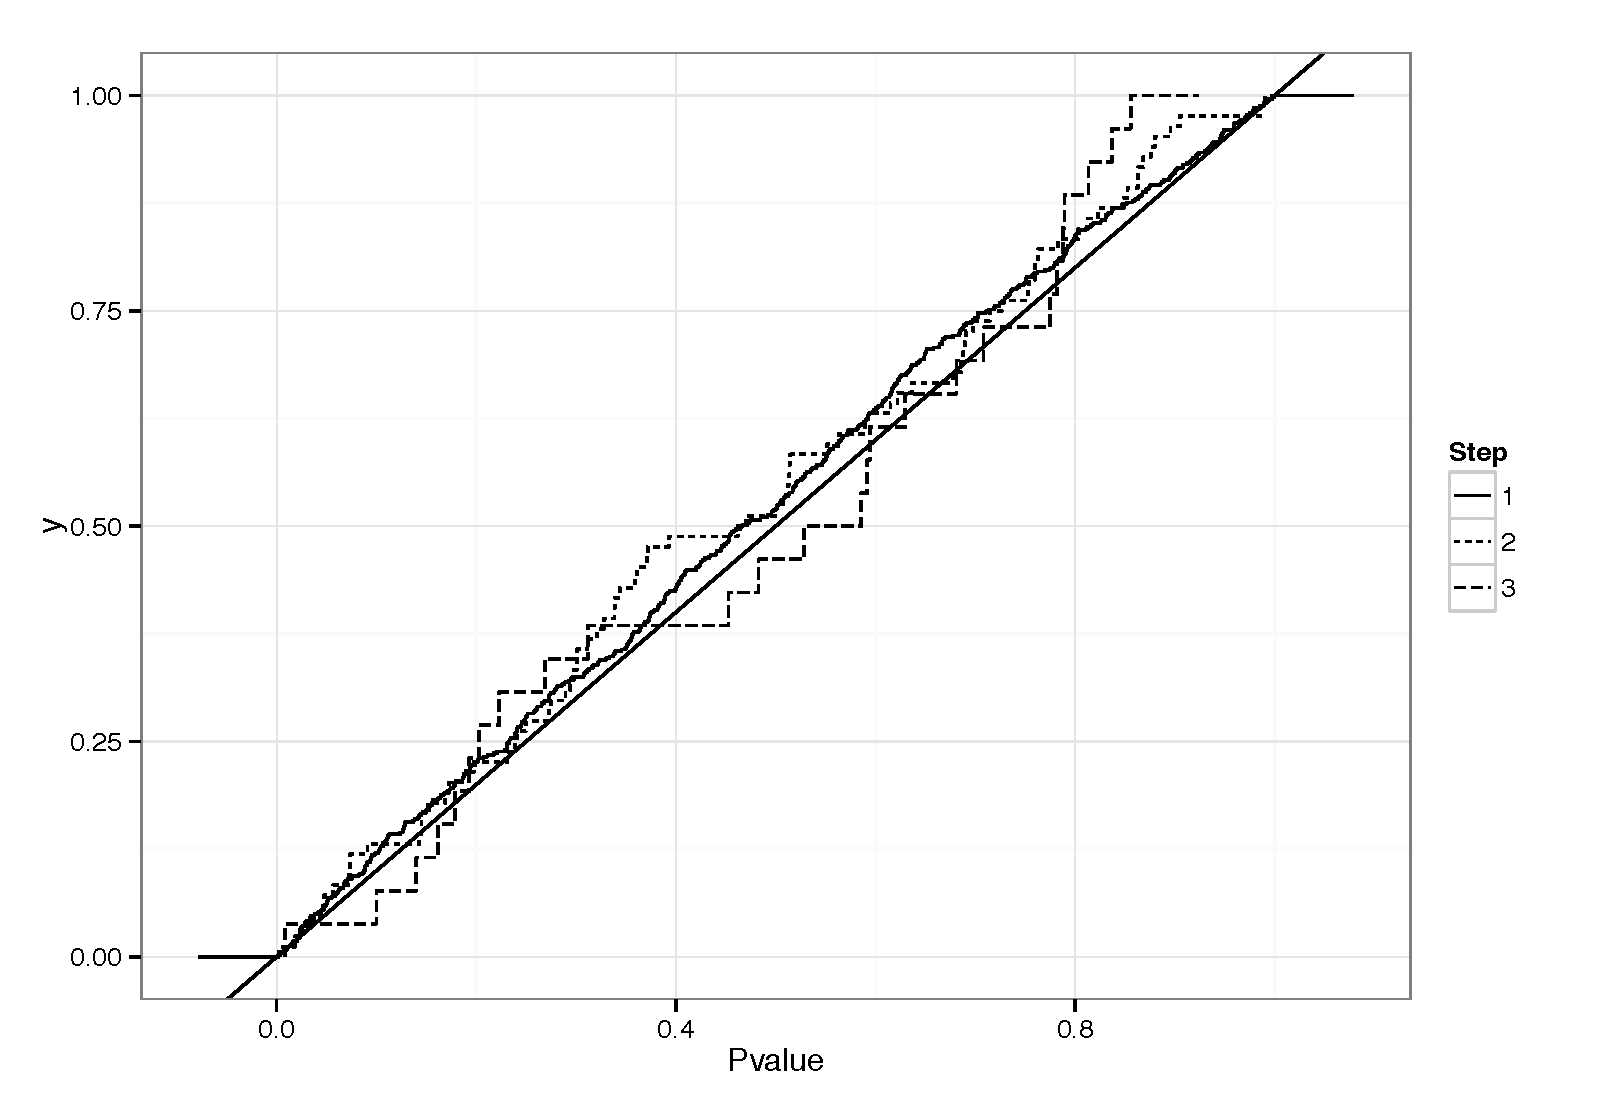
\includegraphics[width=8cm,
    height=8cm]{../../../r/josh/cvresults/results_cv_n50_p100_sparsity0_snr0_bystep.pdf}
    \column{.3\textwidth}
    About 16\% chose sparsity $> 1$ \\ \  \\ Less than 0.5\% chose sparsity $> 3$
  \end{columns}

\end{frame}

\begin{frame}{5-sparse, K = 5, SNR = 7, n = 50, p = 100, steps = 10}
  
  \begin{columns}[c]
    \column{.7\textwidth}
    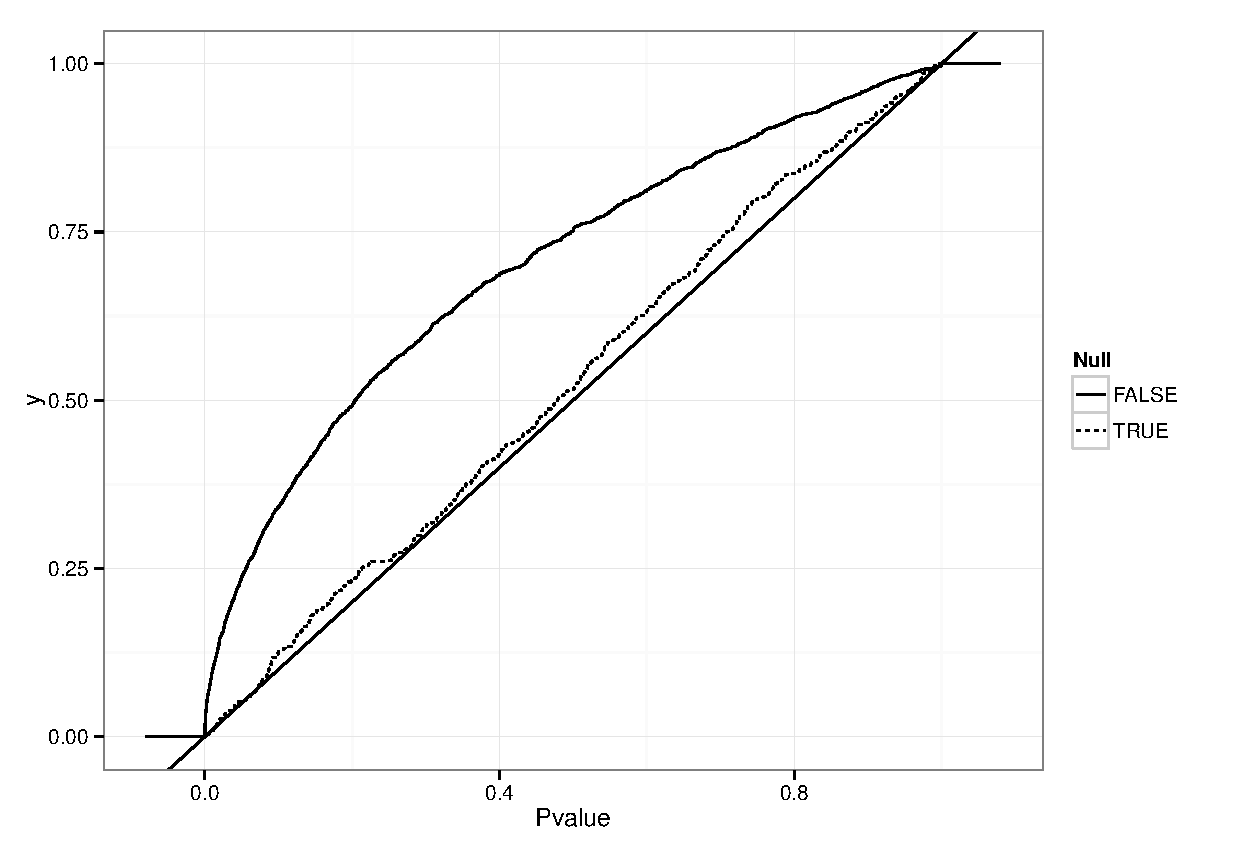
\includegraphics[width=8cm, height=8cm]{../../../r/josh/cvresults/results_cv_n50_p100_sparsity5_snr1_bynull.pdf}
    \column{.3\textwidth}
    Screened 90\% \\ \  \\ Another 4\% 4/5
  \end{columns}
    
\end{frame}

\section{Conclusion}
\label{sec:future}

% \begin{frame}{Limitations / ongoing work}

%   \begin{itemize}

%   \item Forward stepwise used linearity $\hat y^f = P y^{-f}$. Ridge
%     has same form. Lasso has additional constant terms. 

%   \item Computationally very expensive. About 15s for null, 75s for
%     nonnull. Might be able to optimize a little more. 

%   \item Conditioning on too much to reduce dimension? $Z = y -
%     Py$. (Not cross-validation specific, limitation of some
%     selective inference tests). Only about 24\% nonnull were $<
%     0.05$. 

%   \item Tuning parameters: $K$ and $\text{maxsteps}$ (or $\lambda$
%     grid).

%   \item Unknown $\sigma$. Estimate by CV / use selective $F$ test. 

%   \item How to evaluate / plot? (Next slide)

%   \end{itemize}
  
% \end{frame}

\begin{frame}{Messy plots}

    \begin{columns}[c]
      \column{.3\textwidth}
      Summarizing CV results is awkward because the data are not rectangular.
      \column{.7\textwidth}
      \includegraphics[width=8cm, height=8cm]{../../../r/josh/cvresults/results_cv_n50_p100_sparsity5_snr1_bystepnull.pdf}  
    \end{columns}
    
  
\end{frame}

\begin{frame}{The end, for real this time}
  
  Preprint forthcoming. \\

\ 

  Shameless plug: \texttt{selectiveInference} R package available on
  CRAN. \\

\ 

\centering
  {\Huge Thank you! \\ \ \\ \ \\ \ }

%  {\tiny (Don't forget the bonus mystery slide if there is time)}

\end{frame}

% \begin{frame}{Bonus mystery slide}

%     \begin{columns}[c]
%       \column{.5\textwidth}
%       \includegraphics[width=6cm, height=6cm]{../../../r/josh/cvresults/results_cv_n50_p100_sparsity0_snr0_known_reduced.pdf}  
%       \column{.5\textwidth}
%       \includegraphics[width=6cm, height=6cm]{../../../r/josh/cvresults/results_cv_n50_p100_sparsity0_snr0_known.pdf}  
%     \end{columns}  
  
% \end{frame}

\end{document}